\chapter{Projekt aplikacji}
\section{Opis aplikacji}
Aplikacja stworzona na potrzeby przeprowadzenia badań jest serwisem typu \textsl{RESTful}. Jej celem jest przechowywanie danych w bazie w postaci \textsl{klucz-wartość}. Aby móc skorzystać z aplikacji klient musi się autoryzować unikalnym kluczem (\textsl{API key}). Klient posiadający klucz może zapisywać i odczytywać dane. 

Wykorzystywany w aplikacji model składa się z dwóch klas jednakowo odwzorowane na kolekcjach bazy \textsl{MongoDB}. Pierwsza klasa, \textsl{Api}, służy do przechowywania w bazie danych informacji o zarejestrowanych kluczach \textsl{API} (\textsl{API key}). Indeksem głównym w kolekcji jest pole \textsl{key}.

Druga klasa, \textsl{Cache}, jest obiektem służącym do przechowywania danych \textsl{klucz-wartość}, które klient chce przechować w bazie.
Kolekcja \textsl{Cache} posiada trzy indeksy:\begin{itemize}
    \item na pole \textsl{\_id},
    \item na pole \textsl{api}, by wyszukiwanie wszystkich obiektów zapisanych z danym kluczem \textsl{API key} było najszybsze,
    \item na parę pół (\textsl{api}, \textsl{key}), by wyszukiwanie pojedynczych obiektów klienta było jak najszybsze.\end{itemize}
Diagram klas aplikacji przedstawiono na  rysunku \ref{fig:class_diagram}. 
\begin{figure}[!ht]
\centering
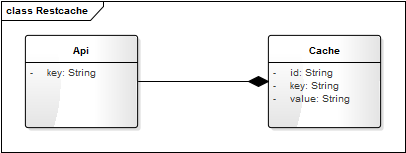
\includegraphics[width=13cm]{\ImgPath/diagram_klas.png}
\caption{Diagram klas aplikacji wykorzystywanej do przeprowadzenia testów}
\label{fig:class_diagram}
\end{figure}

Aplikacje udostępniają \textsl{API}, które przedstawia się w poniżej opisany sposób. Aby otrzymać klucz należy wykonać żądanie \textsl{GET /api/}. W odpowiedzi aplikacja zwróci unikalny, losowy klucz identyfikujący danego klienta. Do generowania kluczy użyty został mechanizm \textsl{UUID} (ang. \textsl{universally unique identifier}) generujący losowy, 128 bitowy ciąg znaków. Przykładowy identyfikator wygląda następująco: \textsl{f0778bae-2902-4ff6-93fa-9776403ecb0f}. W tym momencie klient posiadający swój klucz może tworzyć, aktualizować, usuwać i pobierać obiekty, które są zapisane w bazie danych. Każde żądanie  musi w adresie zawierać otrzymany klucz. Początek żądania ma formę \textsl{/api/\{api\_key\}/}. W przypadku podania błędnego klucza lub jego braku aplikacja zwróci błąd autoryzacji. 
 

Metoda \textsl{GET /api/\{api\_key\}/\{key\}} pozwala na pobranie zapisanej wartości w bazie danych. Jeśli nie istnieje wartość o podanym kluczu zwracany jest błąd \textsl{HTTP 404 - Not Found}. Rysunek \ref{fig:pobieranie_obiektu} prezentuje diagram aktywności dla pobierania obiektu w aplikacji.
\begin{figure}[!ht]
\centering
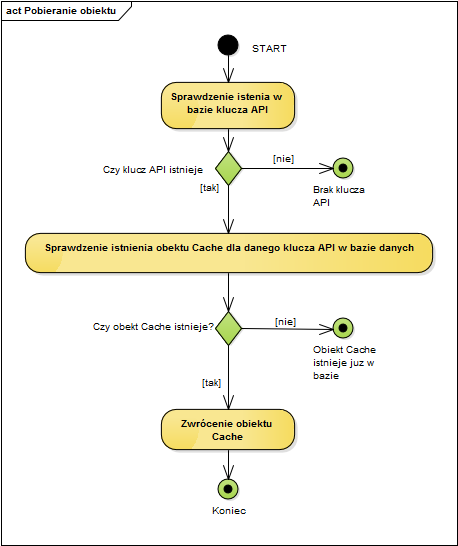
\includegraphics[height=15cm]{\ImgPath/pobieranie_obiektu.png}
\caption{Diagram aktywności pobierania obiektu w aplikacji}
\label{fig:pobieranie_obiektu}
\end{figure}

Metoda \textsl{POST /api/\{api\_key\}/\{key\}} pozwala na utworzenie obiektu \textsl{Cache} w bazie danych. Jeśli w bazie danych istnieje obiekt \textsl{Cache} o podanym kluczu zwracany jest błąd \textsl{HTTP 409 - Conflict}. Natomiast jeśli w przesyłanym żądaniu pole \textsl{value} nie zostanie zdefiniowane lub wartość będzie pusta (\textsl{null}), aplikacja zwróci błąd \textsl{HTTP 400 - Bad request}.  Rysunek \ref{fig:tworzenie_obiektu} prezentuje diagram aktywności dla tworzenia obiektu w aplikacji.
\begin{figure}[!ht]
\centering
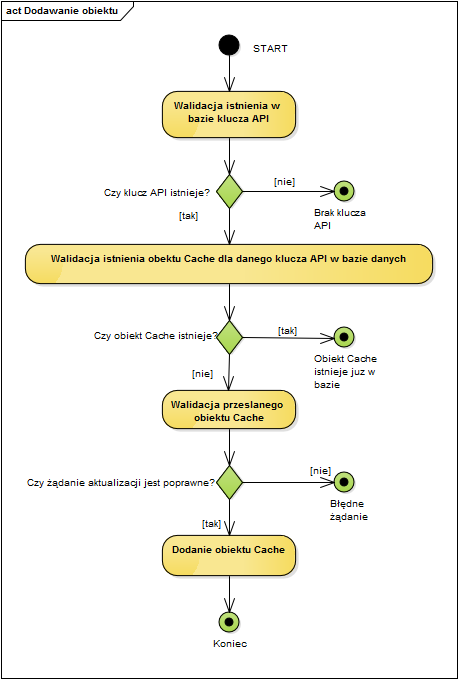
\includegraphics[height=15cm]{\ImgPath/dodawanie_obiektu.png}
\caption{Diagram aktywności tworzenia obiektu w aplikacji}
\label{fig:tworzenie_obiektu}
\end{figure}

Metoda \textsl{PUT /api/\{api\_key\}/\{key\}} pozwala na aktualizacje istniejącego obiektu \textsl{Cache} w bazie danych. Jeśli w bazie danych  nie istnieje obiekt \textsl{Cache} o podanym kluczu zwracany jest błąd \textsl{HTTP 404 - Not Found}, a jeśli w przesyłanym żądaniu pole \textsl{value} nie zostanie zdefiniowane lub wartość będzie pusta (\textsl{null}), aplikacja zwróci błąd \textsl{HTTP 400 - Bad request}. Rysunek \ref{fig:aktualizowanie_obiektu} prezentuje diagram aktywności dla aktualizowania obiektu w aplikacji.
\begin{figure}[!ht]
\centering
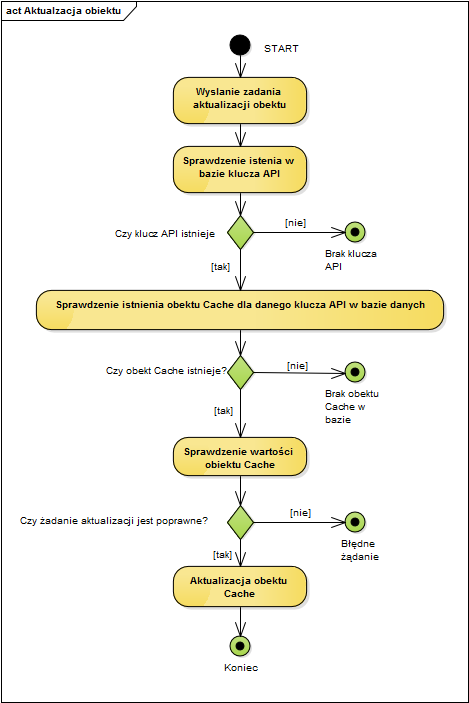
\includegraphics[height=18cm]{\ImgPath/aktualizacja_obiektu.png}
\caption{Diagram aktywności aktualizowania obiektu w aplikacji}
\label{fig:aktualizowanie_obiektu}
\end{figure}

Metoda \textsl{DELETE /api/\{api\_key\}/\{key\}} pozwala na usunięcie istniejącego obiektu \textsl{Cache} z bazy danych. Jeśli w bazie danych  nie istnieje obiekt \textsl{Cache} o podanym kluczu zwracany jest błąd \textsl{HTTP 404 - Not Found}. Rysunek \ref{fig:usuwanie_obiektu} prezentuje diagram aktywności dla usuwanie obiektu w aplikacji.
\begin{figure}[!ht]
\centering
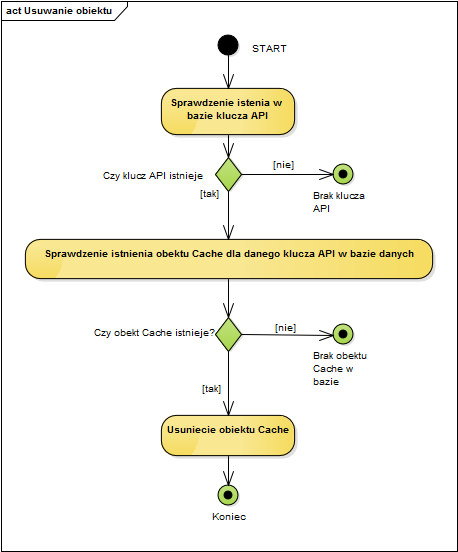
\includegraphics[height=15cm]{\ImgPath/usuwanie_obiektu.png}
\caption{Diagram aktywności usuwanie obiektu w aplikacji}
\label{fig:usuwanie_obiektu}
\end{figure}

Ostatnią dostępną metodą jest żądanie \textsl{GET /api/\{api\_key\}}, które pozwala na pobranie listy wszystkich obiektów, które klient o danym \textsl{api\_key} zapisał.

\section{Testy akceptacyjne} 

By potwierdzić, że stworzone \textsl{API} aplikacji w językach \textsl{Java} i \textsl{Go}  zachowuje się tak samo zostały przygotowane 24 testy akceptacyjne przy użyciu biblioteki \textsl{Spock}, która została opisana w rozdziale \ref{groovy_and_spock}.

W dodatku \ref{sec:acceptance_tests_appendix}  przedstawione rezultaty testów aplikacji uruchomionych na serwerze \textsl{Tomcat} (rysunek \ref{fig:acceptance_test_tomcat}), na serwerze \textsl{Jetty} (rysunek \ref{fig:acceptance_test_jetty}) oraz w języku \textsl{Go} (rysunek \ref{fig:acceptance_test_go}).


